% ------------------------- REVISADO - GRAMATICA - CITAÇÃO
\mychapter{Referencial teórico}
\label{Cap:ReferencialTeorico}

Este capítulo explora a prática da reconciliação de dados, a sua aplicação no âmbito industrial e a utilização da técnica de minimização de multivariáveis pelo método de multiplicadores de Lagrange, que servem como base para o desenvolvimento do \textit{software} apresentado. Além disso, discute-se o desenvolvimento de uma plataforma \textit{web} que proporciona acessibilidade e praticidade para o monitoramento e a manipulação de dados em tempo real. O capítulo contextualiza ainda a sinergia entre a indústria e a internet, destacando o papel essencial que a plataforma \textit{web} desempenha no cenário atual ao integrar técnicas de reconciliação com uma interface intuitiva e acessível.

% ------------------------- REVISADO - GRAMATICA - CITAÇÃO
\section{Reconciliação de dados e método de Lagrange}

% ------------------------- REVISADO - GRAMATICA - CITAÇÃO
\subsection{Definição de reconciliação de dados}

A reconciliação de dados é uma prática utilizada em diversas áreas da ciência e engenharia para assegurar a consistência e precisão dos dados provenientes de diferentes fontes \cite{datarecshakar}. Em contextos como sistemas industriais, processos químicos e redes de sensores, essa técnica é essencial para garantir que os dados coletados estejam alinhados e coerentes. Basicamente, a reconciliação de dados envolve comparar e corrigir discrepâncias entre os valores observados e os valores esperados, com base em modelos e relações matemáticas predefinidas \cite{datarecragnoli}.

Com a evolução dos sistemas automatizados de coleta de dados, como PLCs, sistemas supervisórios e PIMS \cite{plcsupervisory2021}, a captura e o encaminhamento de dados tornaram-se processos eficientes. No entanto, muitos desses dados não satisfazem as equações de balanço, fundamentais em contextos industriais \cite{balance2020}. De acordo com essas equações, em um contorno fechado, a soma das saídas deve ser igual à soma das entradas, subtraindo-se o valor acumulado:

\begin{equation}
	\sum (\text{saídas}) = \sum (\text{entradas}) - \text{armazenado}
\end{equation}

Essa inconsistência geralmente decorre de fatores como erros de medição aleatórios, instrumentos descalibrados, modelagem inadequada e frequências incorretas de amostragem \cite{measurementerror2020}. Outros fatores, como a variação de densidade devido à temperatura e leituras fora da faixa de operação dos instrumentos, também contribuem para esses desvios \cite{temperaturedensity2022}.

Tradicionalmente, os ajustes nos dados baseiam-se em níveis de confiança atribuídos empiricamente a determinadas medições, o que envolve ajustes manuais e subjetivos \cite{empiricaladjustment2023}. No entanto, o presente trabalho busca introduzir uma abordagem matemática para recalcular os valores mais prováveis, eliminando a dependência de ajustes empíricos e subjetivos e promovendo uma análise mais objetiva e fundamentada dos dados industriais \cite{mathematicalapproach2024}.

% ------------------------- REVISADO - GRAMATICA - CITAÇÃO
\subsection{Reconciliação de dados no âmbito industrial}

No começo da década de 1960 se entendeu a importância do controle de processos químicos industriais por computadores que aplicavam técnicas matemáticas \cite{computecontrol}, dessa forma surge a área da computação voltada à reconciliação de dados, na qual há a comparação, validação e correção de informações coletadas em diferentes pontos do processo, a fim de determinar a consistência dos dados, a qualidade dos mesmos ou até otimizar os processos \cite{datarecshakar}.

Ao longo das últimas décadas, os métodos de reconciliação de dados evoluíram significativamente, acompanhando os avanços tecnológicos e as demandas crescentes da indústria \cite{datarecsurvey}. Com o advento de sistemas de automação mais avançados, sensores inteligentes e a proliferação de dispositivos conectados, a quantidade de dados gerados nas operações industriais aumentou drasticamente \cite{datarecsurvey}. Nesse contexto, a reconciliação, análise e gestão de dados tornaram-se ferramentas indispensáveis para garantir a integridade e a confiabilidade das informações coletadas em tempo real \cite{aularecon}.

Na era contemporânea, a reconciliação de dados desempenha um papel crucial na otimização dos processos industriais, contribuindo para a eficiência operacional e a redução de custos. Sistemas avançados de reconciliação não apenas comparam e validam dados, mas também utilizam algoritmos sofisticados para identificar padrões, tendências e anomalias \cite{datarecragnoli}. Essa capacidade analítica permite que as indústrias ajam proativamente, antecipando-se a problemas potenciais, otimizando a produção e melhorando a qualidade dos produtos finais \cite{datarecshakar}.

% ------------------------- REVISADO - GRAMATICA - CITAÇÃO
\subsection{Minimização de multivariáveis por multiplicadores de Lagrange}

A técnica de minimização por multiplicadores de Lagrange foi introduzida por Joseph-Louis Lagrange, um matemático e físico francês nascido em 25 de janeiro de 1736, em Turim, Itália, que mais tarde se estabeleceu na França. Lagrange é conhecido por suas contribuições fundamentais em mecânica analítica, cálculo e teoria dos números, além de desenvolver o método dos multiplicadores de Lagrange no século XVIII, fornecendo uma maneira eficaz de resolver problemas de otimização condicionada \cite{lagrange}.

% ------------------------- REVISADO - GRAMATICA - CITAÇÃO
\subsubsection{O método dos multiplicadores de Lagrange}

O método dos multiplicadores de Lagrange é uma técnica utilizada para encontrar máximos e mínimos de uma função sujeita a uma ou mais restrições. Considera-se o problema de minimizar uma função $f(x, y, z, \dots)$ sujeita a uma restrição $g(x, y, z, \dots) = 0$. Para transformar esse problema com restrições em um problema sem restrições, introduz-se uma variável adicional, o multiplicador de Lagrange, que representa o impacto da restrição sobre a função objetivo. Em um problema de minimização com uma única restrição, a função de Lagrange $\mathcal{L}$ é definida como mostrado na Equação \ref{eq
}:

\begin{equation} \mathcal{L}(x, y, z, \dots, \lambda) = f(x, y, z, \dots) + \lambda \cdot g(x, y, z, \dots) \label{eq
} \end{equation}

onde $\lambda$ é o multiplicador de Lagrange.

A solução do problema ocorre ao determinar os pontos críticos de $\mathcal{L}$, isto é, os pontos onde as derivadas parciais de $\mathcal{L}$ em relação a todas as variáveis (incluindo $\lambda$) são iguais a zero. Portanto, é necessário resolver o sistema de equações conforme apresentado na Equação \ref{eq:lambdaa}:

\begin{equation} \frac{\partial \mathcal{L}}{\partial x} = 0, \quad \frac{\partial \mathcal{L}}{\partial y} = 0, \quad \frac{\partial \mathcal{L}}{\partial z} = 0, \quad \dots, \quad \frac{\partial \mathcal{L}}{\partial \lambda} = 0 \label{eq:lambdaa} \end{equation}

% ------------------------- REVISADO - GRAMATICA - CITAÇÃO
\subsubsection{Exemplo com duas variáveis}

Considera-se o caso de uma função de duas variáveis, $f(x, y)$, que necessita ser minimizada sujeita a uma restrição $g(x, y) = 0$. A função de Lagrange é dada por:

\begin{equation}
	\mathcal{L}(x, y, \lambda) = f(x, y) + \lambda \cdot g(x, y)
	\label{eq:lagrange_two_variable}
\end{equation}

Para encontrar os valores de $x$, $y$ e $\lambda$ que minimizam $f(x, y)$, resolve-se o sistema de equações apresentado nas Equações \ref{eq:partial_x}, \ref{eq:partial_y} e \ref{eq:partial_lambda}, conforme mostrado a seguir:

\begin{equation}
	\frac{\partial \mathcal{L}}{\partial x} = \frac{\partial f}{\partial x} + \lambda \frac{\partial g}{\partial x} = 0
	\label{eq:partial_x}
\end{equation}
\begin{equation}
	\frac{\partial \mathcal{L}}{\partial y} = \frac{\partial f}{\partial y} + \lambda \frac{\partial g}{\partial y} = 0
	\label{eq:partial_y}
\end{equation}
\begin{equation}
	\frac{\partial \mathcal{L}}{\partial \lambda} = g(x, y) = 0
	\label{eq:partial_lambda}
\end{equation}

A resolução desse sistema fornece os valores de $x$, $y$ e $\lambda$ que minimizam $f(x, y)$ enquanto satisfazem a restrição $g(x, y) = 0$.

O método dos multiplicadores de Lagrange é amplamente utilizado em diversas áreas, incluindo otimização de processos industriais, economia e física, onde os problemas frequentemente envolvem restrições complexas. A abordagem permite uma solução sistemática e rigorosa para problemas de otimização condicionada, assegurando que as soluções encontradas respeitem as restrições impostas \cite{lagrangeoptbook}.

% ------------------------- REVISADO - GRAMATICA - CITAÇÃO
\subsection{Aplicação do método dos multiplicadores de Lagrange à necessidade de reconciliação de dados}

Para resolver o problema de balanço de massas, o método dos multiplicadores de Lagrange é aplicado adotando o critério dos mínimos quadrados. Define-se uma função objetivo a ser minimizada, que corresponde à soma ponderada dos quadrados dos erros nas medições.

Seja $M_i$ o valor medido de um fluxo e $\hat{M}_i$ o valor corrigido para o mesmo fluxo. O erro $E_i$ é então definido como a diferença entre esses valores, conforme a Equação \ref{eq:definition}:
\begin{equation}
	E_i = M_i - \hat{M}_i
 \label{eq:definition}
\end{equation}

O erro quadrático correspondente é dado pela Equação \ref{eq:quadratic_error}:
\begin{equation}
	E_i^2 = (M_i - \hat{M}_i)^2
    \label{eq:quadratic_error}
\end{equation}

Para ponderar cada erro, utiliza-se o inverso do desvio padrão associado à medida. A função objetivo, portanto, é formulada da seguinte maneira, como demonstrado na Equação \ref{eq:def_lagre1}:
\begin{equation}
	F(\hat{M}_1, \hat{M}_2, \dots, \hat{M}_n) = \sum_{i=1}^n \frac{(M_i - \hat{M}_i)^2}{\sigma_i^2}
     \label{eq:def_lagre1}
\end{equation}

As restrições para o problema são expressas pela Equação \ref{eq:def_lagre2}:
\begin{equation}
	\phi_j(\hat{M}_1, \hat{M}_2, \dots, \hat{M}_n) = 0, \quad j = 1, 2, \dots, m
     \label{eq:def_lagre2}
\end{equation}
onde cada $\phi_j$ representa uma equação de balanço de massa para um nó do circuito, totalizando $m$ equações de restrição.

A função de Lagrange, que incorpora essas restrições, é então definida pela Equação \ref{eq:def_lagre3}:
\begin{equation}
	\Phi = \sum_{i=1}^n \frac{(M_i - \hat{M}_i)^2}{\sigma_i^2} + \sum_{j=1}^m \lambda_j \phi_j(\hat{M}_1, \hat{M}_2, \dots, \hat{M}_n)
     \label{eq:def_lagre3}
\end{equation}

Calculando as derivadas parciais de $\Phi$ em relação a cada variável corrigida $\hat{M}_i$ e igualando a zero, obtêm-se um conjunto de $n$ equações para cada medida, como mostrado na Equação \ref{eq:measure_equation}:
\begin{equation}
	\frac{\partial \Phi}{\partial \hat{M}_1} = 0, \quad \frac{\partial \Phi}{\partial \hat{M}_2} = 0, \quad \dots, \quad \frac{\partial \Phi}{\partial \hat{M}_n} = 0
     \label{eq:measure_equation}
\end{equation}

Juntas com as $m$ equações de restrição $\phi_j = 0$, essas expressões formam um sistema de $n + m$ equações para $n + m$ incógnitas, permitindo a resolução para determinar os valores reconciliados das variáveis.

% ------------------------- REVISADO - GRAMATICA - CITAÇÃO
\subsubsection{Exemplo com um problema de balanço de sistema}
Para ilustrar a aplicação do método dos multiplicadores de Lagrange na reconciliação de dados, considera-se um problema de balanço de um sistema com o número de medições \(N = 3\) e o número de nódulos \(H = 1\), conforme descrição e detalhamento das notas de aula de SEIXAS, Constantino (2005), descrito na Figura \ref{Fig:ExemploImage}.

\begin{figure}[htbp]
    \centering
    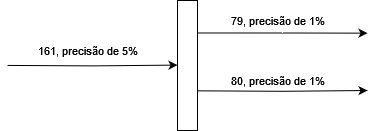
\includegraphics[width=0.6\textwidth]{figuras/exemplo-problema.png}
    \caption{Um exemplo com medidas (Fonte: próprio autor, 2024).}
    \label{Fig:ExemploImage}
\end{figure}

O vetor de medições \(m\) é dado pela Equação \eqref{eq:medidas}:
\begin{equation}
    m = [M_1 \quad M_2 \quad M_3] = [161 \quad 79 \quad 80]
    \label{eq:medidas}
\end{equation}

O vetor de desvios percentuais \(p\) é expresso na Equação \eqref{eq:desvios_percentuais}:
\begin{equation}
    p = [\sigma_1 \quad \sigma_2 \quad \sigma_3] = [0.05 \quad 0.01 \quad 0.01]
    \label{eq:desvios_percentuais}
\end{equation}

Para calcular o vetor de desvios absolutos \(a\), utiliza-se a notação do Matlab, realizando a operação elemento a elemento entre o vetor de medições e o vetor de desvios percentuais, conforme demonstrado na Equação \eqref{eq:desvios_absolutos}:
\begin{equation}
    a = m .* p = [8.05 \quad 0.79 \quad 0.80]
    \label{eq:desvios_absolutos}
\end{equation}

Para facilitar a implementação do cálculo de reconciliação, o sistema é formulado em notação matricial. A Equação \eqref{eq:sistema_matricial} representa o sistema de equações utilizado:

\begin{equation}
\begin{bmatrix}
    \frac{2}{a_1^2} & 0 & 0 & 1 \\
    0 & \frac{2}{a_2^2} & 0 & -1 \\
    0 & 0 & \frac{2}{a_3^2} & 1 \\
    1 & -1 & -1 & 0 \\
\end{bmatrix}
\begin{bmatrix}
    \hat{M}_1 \\
    \hat{M}_2 \\
    \hat{M}_3 \\
    \lambda_1 \\
\end{bmatrix}
=
\begin{bmatrix}
    \frac{2 M_1}{a_1^2} \\
    \frac{2 M_2}{a_2^2} \\
    \frac{2 M_3}{a_3^2} \\
    0 \\
\end{bmatrix}
\label{eq:sistema_matricial}
\end{equation}

A resolução do sistema, conforme mostrado na Equação \eqref{eq:sistema_resolvido}, é realizada invertendo a matriz e multiplicando-a pelo vetor dos termos independentes:

\begin{equation}
\begin{bmatrix}
    \hat{M}_1 \\
    \hat{M}_2 \\
    \hat{M}_3 \\
    \lambda_1 \\
\end{bmatrix}
=
\begin{bmatrix}
    \frac{2}{a_1^2} & 0 & 0 & 1 \\
    0 & \frac{2}{a_2^2} & 0 & -1 \\
    0 & 0 & \frac{2}{a_3^2} & 1 \\
    1 & -1 & -1 & 0 \\
\end{bmatrix}^{-1}
\begin{bmatrix}
    \frac{2 M_1}{a_1^2} \\
    \frac{2 M_2}{a_2^2} \\
    \frac{2 M_3}{a_3^2} \\
    0 \\
\end{bmatrix}
\label{eq:sistema_resolvido}
\end{equation}

O vetor de correções, que representa as diferenças entre as medições originais e os valores reconciliados, é definido pela Equação \eqref{eq:vetor_correcoes}:

\begin{equation}
\begin{bmatrix}
    E_1 \\
    E_2 \\
    E_3 \\
\end{bmatrix}
=
\begin{bmatrix}
    M_1 \\
    M_2 \\
    M_3 \\
\end{bmatrix}
-
\begin{bmatrix}
    \hat{M}_1 \\
    \hat{M}_2 \\
    \hat{M}_3 \\
\end{bmatrix}
\label{eq:vetor_correcoes}
\end{equation}

O resultado final das medidas reconciliadas é apresentado na Equação \eqref{eq:medidas_reconciliadas}:

\begin{equation}
    Rec = [159.0383 \quad 79.0189 \quad 80.0194]
    \label{eq:medidas_reconciliadas}
\end{equation}

A correção dos valores, ou seja, a variação entre o valor medido e o valor reconciliado, é descrita na Equação \eqref{eq:correcao_valores}:

\begin{equation}
    E = [1.9617 \quad -0.0189 \quad -0.0194 ]
    \label{eq:correcao_valores}
\end{equation}



% ------------------------- REVISADO - GRAMATICA - CITAÇÃO
\section{Desenvolvimento de um \textit{software online}}

O desenvolvimento de \textit{softwares} online modernos requer uma abordagem estruturada que combina diferentes áreas de conhecimento, como \textit{front-end}, \textit{back-end} e gerenciamento de banco de dados. Esses componentes trabalham em conjunto para criar sistemas robustos, escaláveis e acessíveis, fundamentais para atender às demandas de aplicações na \textit{web}.

% ------------------------- REVISADO - GRAMATICA - CITAÇÃO
\subsection{Desenvolvimento \textit{front-end}}

O \textit{front-end} é a camada de uma aplicação com a qual os usuários interagem diretamente. Ele compreende os elementos visíveis e interativos da interface, como botões, menus, e formulários, e é fundamental para proporcionar uma experiência de uso intuitiva e eficiente \cite{frontendrole}. O desenvolvimento de um \textit{front-end} eficaz exige atenção tanto à organização visual quanto à responsividade, garantindo que a aplicação funcione bem em diferentes dispositivos e tamanhos de tela.

Para o desenvolvimento \textit{front-end}, existem diversas linguagens e \textit{frameworks} amplamente utilizados. HTML, CSS e JavaScript são as linguagens fundamentais para a construção de interfaces web. Entre os \textit{frameworks} e bibliotecas mais populares estão \textit{React}, \textit{Vue.js} e \textit{Angular}, que oferecem ferramentas avançadas para criar interfaces de usuário dinâmicas e reativas \cite{reactbook}. Além disso, \textit{frameworks} de estilo como \textit{Bootstrap} e \textit{Tailwind CSS} auxiliam no \textit{design} responsivo e na organização visual das páginas \cite{bootstrapdoc}.

No desenvolvimento do RADARE, a construção da interface foi realizada utilizando \textit{TypeScript} em conjunto com HTML e SCSS, proporcionando uma base sólida para a criação de interfaces organizadas e responsivas \cite{typescriptbook}. O HTML foi utilizado para estruturar os elementos visuais da interface, enquanto o SCSS garantiu um controle avançado sobre o \textit{design} e o estilo, permitindo uma customização precisa de cada componente \cite{htmlcssbook}. A escolha do \textit{TypeScript} trouxe benefícios como tipagem estática e maior segurança no desenvolvimento, facilitando a criação de uma interface robusta e escalável \cite{typescriptsecurity}. Diferente do uso de \textit{frameworks} de \textit{front-end}, que adicionam camadas adicionais de abstração, a combinação direta dessas tecnologias possibilitou um controle detalhado sobre a interface e a experiência do usuário \cite{frontendwithoutframework}.

% ------------------------- REVISADO - GRAMATICA - CITAÇÃO
\subsection{Desenvolvimento \textit{back-end}}

O \textit{back-end} de uma aplicação é a parte que opera "por trás dos panos", onde toda a lógica de negócios, manipulação de dados e comunicação com o banco de dados ocorre. Essa camada é fundamental para o funcionamento adequado do sistema, pois realiza operações como autenticação, processamento de dados e execução de cálculos específicos, garantindo que as informações exibidas no \textit{front-end} estejam sempre atualizadas e em conformidade com as regras de negócio definidas \cite{backendroles}.

Entre as linguagens mais utilizadas para o desenvolvimento de \textit{back-end} estão \textit{Python}, \textit{Java}, \textit{Ruby}, \textit{PHP}, e \textit{Node.js}. Cada uma delas possui características específicas que se adequam a diferentes tipos de aplicações e requisitos de desempenho, escalabilidade e manutenção \cite{backendlanguages}. Por exemplo, a linguagem \textit{Python} é amplamente apreciada por sua sintaxe clara e suporte a bibliotecas de manipulação de dados, enquanto \textit{Java} é conhecida por sua robustez e escalabilidade em grandes sistemas empresariais \cite{javabackend}.

No desenvolvimento do RADARE, o \textit{back-end} foi inteiramente construído utilizando a linguagem \textit{Python}, que permite a implementação de uma estrutura eficiente para manipulação de dados e integração com o \textit{front-end} \cite{pythonweb}. Com a \textit{Python}, é possível desenvolver APIs que facilitam a comunicação entre a interface de usuário e o sistema de armazenamento de dados, garantindo uma troca eficiente de informações e a consistência dos dados processados \cite{pythonapi}. A linguagem também forneceu um ambiente propício para lidar com a lógica de reconciliação de dados, pois realiza operações necessárias de forma otimizada e segura \cite{pythondata}.

Por meio dessa abordagem, o \textit{back-end} do RADARE é capaz de processar dados de entrada, realizar cálculos de reconciliação e enviar os resultados para o \textit{front-end} de maneira integrada \cite{backendworkflow}. Esse uso exclusivo de \textit{Python} como linguagem \textit{back-end} trouxe simplicidade e consistência ao sistema, atendendo aos requisitos do projeto com robustez e flexibilidade.

% ------------------------- REVISADO - GRAMATICA - CITAÇÃO
\subsection{Desenvolvimento do banco de dados}

Um banco de dados é uma coleção organizada de informações estruturadas, geralmente armazenadas e acessadas eletronicamente a partir de um sistema de computador. Em sistemas modernos, os bancos de dados são essenciais para armazenar, recuperar e gerenciar grandes volumes de dados de maneira rápida e eficiente. Eles desempenham um papel central em aplicações \textit{online}, onde a integridade, consistência e segurança dos dados são fundamentais.

Existem diferentes tipos de bancos de dados, cada um projetado para atender a requisitos específicos de armazenamento e acesso. Entre os modelos mais comuns estão dois:

\begin{itemize}
	\item \textbf{Bancos de dados relacionais (SQL)}: Organizam os dados em tabelas com linhas e colunas, permitindo consultas complexas através da linguagem SQL. Exemplos incluem \textit{PostgreSQL}, \textit{MySQL} e \textit{Oracle Database} \cite{relationaldatabases}.

	\item \textbf{Bancos de dados não relacionais(NoSQL)}: Projetados para armazenamento flexível de dados não estruturados ou semi-estruturados, esses bancos de dados não utilizam a estrutura tradicional de tabelas. São divididos em subcategorias como \textit{document stores} (ex.: \textit{MongoDB}), \textit{key-value stores} (ex.: \textit{Redis}), \textit{column stores} (ex.: \textit{Cassandra}) e \textit{graph databases} (ex.: \textit{Neo4j}) \cite{nosqldatabases}.
\end{itemize}

No desenvolvimento do RADARE, o banco de dados foi implementado utilizando exclusivamente o \textit{PostgreSQL}, um sistema de gerenciamento de banco de dados relacional robusto e altamente confiável \cite{postgresql2024}. O \textit{PostgreSQL} foi escolhido por sua capacidade de gerenciar grandes volumes de dados e por oferecer suporte a transações complexas, garantindo a integridade e consistência das informações armazenadas \cite{acidtransactions}.

O \textit{PostgreSQL} organiza os dados em tabelas relacionais, onde cada linha e coluna representam uma entidade específica e suas respectivas propriedades, facilitando a execução de consultas e manipulações complexas \cite{relationaldatabases}. Além disso, o sistema fornece mecanismos de integridade referencial, que ajudam a manter a consistência dos dados por meio de relações entre tabelas \cite{databaseintegrity}. Essa estrutura é essencial para a reconciliação de dados, uma vez que permite organizar e recuperar informações de forma rápida e precisa.

% ------------------------- REVISADO - GRAMATICA - CITAÇÃO
\subsection{Metodologias de desenvolvimento de \textit{software}}

O desenvolvimento de \textit{software} moderno conta com metodologias específicas que auxiliam na organização, planejamento e execução dos projetos, permitindo maior controle sobre prazos, custos e qualidade do produto final. Entre as metodologias mais utilizadas estão as abordagens ágeis, que buscam otimizar a comunicação entre as equipes e permitir a adaptação contínua aos requisitos do cliente ao longo do ciclo de desenvolvimento.

\begin{itemize} \item \textbf{Agile}: Agile é uma abordagem de desenvolvimento de \textit{software} que se concentra na flexibilidade e na capacidade de adaptação rápida a mudanças nos requisitos \cite{agilemanif}. A metodologia foi formalizada pelo Manifesto Agile em 2001, propondo valores como colaboração com o cliente, resposta a mudanças e entrega contínua de \textit{software} funcional. Em vez de desenvolver o produto como um todo, as equipes Agile dividem o projeto em pequenos incrementos, denominados \textit{sprints}, para gerar valor continuamente ao cliente \cite{agilepractices}.

    \item \textbf{Scrum}: Scrum é uma estrutura dentro da metodologia Agile que organiza o desenvolvimento em \textit{sprints} de curta duração, geralmente de duas a quatro semanas \cite{scrumguide}. Durante cada \textit{sprint}, a equipe trabalha em um conjunto específico de tarefas, definido em uma reunião de planejamento. Ao final de cada ciclo, ocorre uma reunião de revisão onde o progresso é avaliado e ajustes são feitos para o próximo \textit{sprint}. O Scrum enfatiza papéis específicos, como o \textit{Scrum Master} e o \textit{Product Owner}, para manter a equipe focada e produtiva \cite{scrumroles}.

	\item \textbf{Kanban}: Kanban é uma metodologia visual que utiliza um quadro dividido em colunas para representar o fluxo de trabalho, permitindo a gestão e otimização das tarefas \cite{kanbanmethod}. Com foco na melhoria contínua e na redução de desperdícios, o Kanban permite que a equipe ajuste a quantidade de trabalho em progresso para evitar sobrecarga. Essa metodologia é particularmente útil em ambientes onde as tarefas variam constantemente e é necessária uma alta adaptabilidade \cite{kanbanflow}.

	\item \textbf{Extreme Programming (XP)}: O XP é uma metodologia que enfatiza a excelência técnica e práticas rigorosas de desenvolvimento, como programação em par, desenvolvimento orientado a testes (TDD) e integração contínua \cite{extremeprogramming}. O XP visa melhorar a qualidade do \textit{software} e a capacidade de resposta a mudanças, focando na colaboração constante com o cliente e em entregas frequentes de pequenas funcionalidades \cite{tddxp}.

\end{itemize}

Essas metodologias oferecem ferramentas e práticas que ajudam as equipes de desenvolvimento a gerenciar e controlar o progresso dos projetos de \textit{software}, permitindo entregas consistentes e satisfatórias para os clientes. A escolha de uma metodologia específica depende dos requisitos do projeto, da estrutura da equipe e da cultura organizacional, sendo fundamental para o sucesso e a qualidade do produto final.

% ------------------------- REVISADO
\section{A sinergia entre a indústria e a internet}

O panorama atual de avanço da internet e a convergência entre a internet e o setor industrial representam um marco significativo na era da Engenharia de Computação \cite{industry4status}. Este fenômeno transformador tem sido impulsionado pela fusão das tecnologias da informação com os processos industriais, dando origem a conceitos como Indústria 4.0.

No âmbito desta ferramenta, é aplicada a intersecção dessas duas esferas, onde os conceitos de práticas industriais, reconciliação, análise e qualidade de dados se integram à internet, na qual é extraído deles o seu maior forte, como uma maior integralidade com outros sistemas por meio de APIs (interfaces de programação de aplicativos), melhor interatividade entre os elementos do sistema, promovendo uma comunicação mais dinâmica e eficaz, aumento da eficiência operacional e facilidade na gestão de processos \cite{industry4}. Essa sinergia possibilita a criação de ecossistemas industriais mais conectados nos quais os dados relevantes podem ser tratados de forma segura e eficiente. \cite{industrybuild}.

O horizonte atual, delineado pelos recentes avanços tecnológicos e inovações sustenta a perspectiva otimista que as indústrias estão destinadas a experimentar um crescimento substancial no país \cite{industrychina}. A convergência entre a internet e o setor industrial representa um catalisador significativo para a modernização e eficiência operacional. A integração de práticas avançadas de desenvolvimento de soluções voltadas à usabilidade e ao ambiente de desenvolvimento com controle computacional, como a reconciliação de dados e análise preditiva, impulsiona a qualidade e consistência dos processos produtivos \cite{industrydigital}.

Além disso, a aplicação da internet nas práticas industriais não só fortalece a competitividade das empresas, mas também desempenha um papel crucial na expansão econômica do país \cite{industryiot}. A capacidade de adotar tecnologias inovadoras como a automação avançada, coloca as indústrias em uma posição estratégica para atender às crescentes demandas do mercado e elevar a produtividade \cite{industryinternet}. Nesse sentido é plausível afirmar que, diante do atual cenário tecnológico e das tendências emergentes, a ferramenta desenvolvida nesse trabalho tem um grande potencial para aplicação industrial e que pode ajudar a solucionar um problema existente.